

\section{Class-Conditional Sampling} \label{sec:5.1}
Class-conditional sampling works in the same way as semantic synthesis sampling but in general is much easier to do as there is only one label per image instead of one label per pixel. As we will see, the quality of the resulting samples heavily depend on how good the classification network or the segmentation network perform on high noise and in general it is easier to estimate a label from a noisy image than a label for every pixel, where each pixel is transformed by noise up to two magnitudes higher than the individual pixel information.

That SGMs can do class-conditional sampling has been already shown in \cite{score_3} but this capability was exclusively shown for an implementation in Tensorflow. To close this gap we ported the Tensorflow implementation to PyTorch. As a classification network a noise-conditional Wide Residual Network \cite{wrn} was used. 

Interestingly we found that the gradients computed on the WideResNet prediction were around $1000$ times smaller than the gradients of the score-model. Therefore the class-conditional gradients had no effect on the image generation and had to be scaled with an experimentally motivated factor of $1000$ in order to get good results. Since there was not such a scaling factor in the Tensorflow implementation, we would have been very interested to know if the class-conditional gradients in this implementation were larger natively. Unfortunately due to Tensorflows jit (just in time) technique, there is no way to read out any tensors during runtime. As it turns out, these scaling factors are also important in later experiments and must be determined individually for each dataset. Also, it is often not sufficient to choose a static scaling factor, but a scaling factor described by a function must be chosen.

As a qualitative proof of concept we test the implementation on the MNIST \cite{mnist} dataset, which contains handwritten digits in the range $0-9$ and was initially designed for handwriting recognition. Some of our results are shown in \hyperref[fig:5.1]{Fig.\,5.1}. We can conclude that the implementation works in general, although there are some samples that strongly deviate from the requested numbers. This is very likely due to the fact that for the implementation a very basic model and SDE were used. In further experiments the significantly more complicated NCSN++ model and the VE SDE were deployed.
%
\begin{figure}
    \begin{subfigure}{0.3\textwidth} \label{abb:1a}
        \centering
        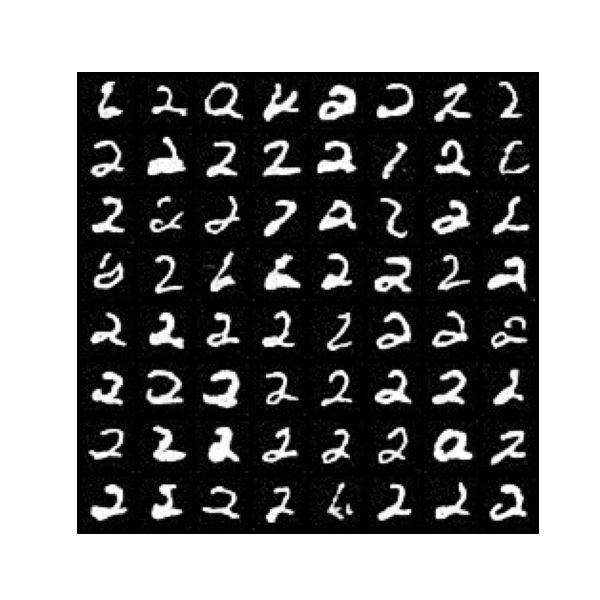
\includegraphics[width=\textwidth]{Chapters/figures/experiments/mnist/mnist_2.png}
    \end{subfigure}
    \begin{subfigure}{0.3\textwidth} \label{abb:1a}
        \centering
        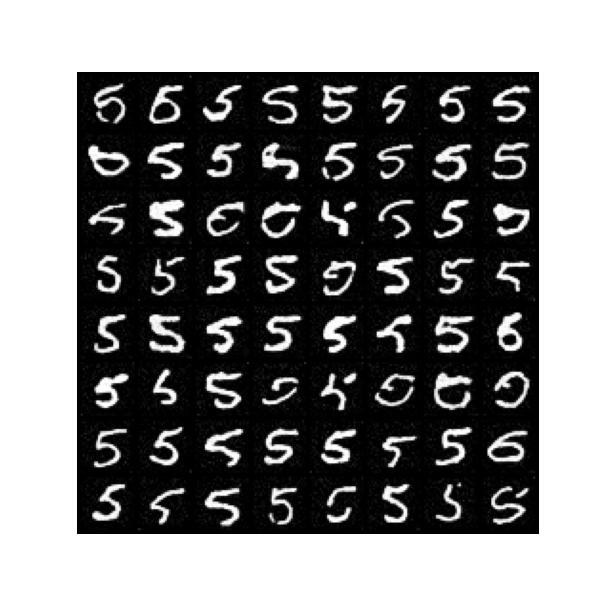
\includegraphics[width=\textwidth]{Chapters/figures/experiments/mnist/mnist_5.png}
    \end{subfigure}
    \begin{subfigure}{0.3\textwidth} \label{abb:1a}
        \centering
        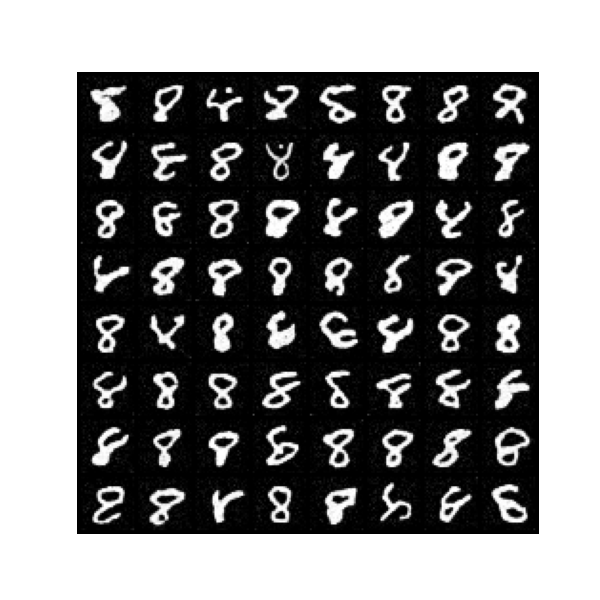
\includegraphics[width=\textwidth]{Chapters/figures/experiments/mnist/mnist_8.png}
    \end{subfigure}
    
    \caption{MNIST class-conditional results. \textit{Left:} 2, \textit{Middle:} 5, \textit{Right:} 8}
    \label{fig:my_label}
\end{figure}
%

%%%%%%%%%%%%%%%%%%%%%%%%%%%%%%%%%%%%%%%%%%%%%%%%%%%%%%%%%%%%%%%%%%%%%%%%%%%%%%%%%%%%%%%%%
\section{Semantic Synthesis Implementation} 
As described in \hyperref[sec:4.5]{Sec.\,4.5} a semantic segmentation network is needed to learn the forward process $\log p_t(\vec{y}|\vec{x}(t))$ which can be then used to solve the $\vec{y}$-dependent reverse SDE in \hyperref[equ:4.22]{Equ.\,4.22}. Effectively this means that the semantic segmentation is learned on noisy images $\vec{x(t)}$, where the noise for timestep $t$ is governed by the forward SDE. Since for each training image $\vec{x}(0)$ there also is a segmentation map $\vec{y}$, the guess $\tilde{\vec{y}}$ of the segmentation network can be compared to the true map to then compute an error. 

\subsection{Generating noisy training images}

As mentioned above – because the forward SDE is tractable – we can easily generate as much noisy training images as we want by adding noise to the initial training images $\{\vec{x}_i(0)\}_{i=1}^N$:
%
\begin{equation} \label{equ:5.1}
    \vec{x}(t)=\vec{x}(0)+\sigma(t)\cdot\vec{z}\,.
\end{equation}
%
In \hyperref[equ:5.1]{Equ.\,5.1} $\vec{z}\sim\mathcal{N}(0, \vec{I})$ is Gaussian noise and $\sigma(t)$ is the noise scale for timestep $t$ which for the VE SDE is given by
%
\begin{equation} \label{5.2}
    \sigma(t)=\sigma_{min}\cdot\left(\frac{\sigma_{max}}{\sigma_{min}}\right)^t.
\end{equation}
%
$\sigma_{min}$ corresponds to $\sigma(t=0)$ and is always chosen as $0.01$. Since the image information is in the range $[0,1]$, a noise of $0.01$ is not visible to the human eye. $\sigma_{max}$ corresponds to $\sigma(t=T\triangleq1)$ and is chosen as the maximum pairwise distance for the dataset under investigation. During training, for each not noisy training image in a batch we then randomly choose noise scales $\sigma(t)$ with $t\in[0,1]$ and transform the not noisy training batch into a noisy training batch by using \hyperref[equ:5.1]{Equ.\,5.1}.

\subsection{Choosing a noise encoding}

With the noisy images we can now train a semantic segmentation network. Obviously a semantic segmentation network is expected to perform increasingly worse on increasingly noisy images. To give an idea of the difficulty of the task, the maximum noise scale for the Cityscapes dataset is $338$, i.e. in images with maximum noise, the noise is $338$ higher than the underlying image information! Therefore, we cannot simply train a regular segmentation network $p_\theta(\vec{x(t)})$ on noisy images, but we need to condition the network on noise $p_\theta(\vec{x}(t), \sigma(t))$, so that it can better distinguish the noise scales. There are some advanced ways to encode this noise information, including \textit{Sinusoidal Positional Embeddings} \cite{attention} or \textit{Gaussian Fourier Embeddings} \cite{fourfeat}. These encoding techniques are used in NCSN++ to encode the noise information but for the segmentation network, we work with a much simpler type of encodings.

Our idea to condition the semantic segmentation is to encode the noise information as a $4th$ channel dimension in addition to the $3$ color channels for each pixel. The size of a batch of (noisy) training image has the size $N\times C\times H\times W$. We want to expand the noise information of size $N$ to size $N\times 1\times H\times W$ and than concatenate the noise with the images to obtain a resulting batch of size $N\times (C+1)\times H\times W$. This batch is then fed into the network.

However, there are several plausible options to express the noise of an image. The first option would be to use the noise scale itself, the second option would be to use the logarithm of the noise scale and the third option would be to use the timestep which directly correlates to noise. Recalling to the noise function in \hyperref[equ:5.2]{Equ.\,5.2} we can plot these three options in \hyperref[fig:5.2]{Fig.\,5.2}.

In order to evaluate these possibilities one needs to know the input format of the images into the network. Normally the pixel values are displayed in the range $[0, 1]$ rather than in the range $[0, 255]$. But since there is noise added to the initial images the pixel ranges can be everywhere from $[0,\sigma_{min}]$ and $[0, \sigma_{max}]$, depending on the current noise scale. When we tried to learn a segmentation network from images in various pixel ranges we got devastating results. Therefore we transform any perturbed image $\vec{x}(t)$ into the range $[0, 1]$ by using the following formula:
%
\begin{equation}
    \vec{x}_{[0,1]}(t)=\frac{\vec{x}(t)-\min(\vec{x}(t))}{\max(\vec{x}(t))-\min(\vec{x}(t))}.
\end{equation}
%

It is plausible that the noise encodings should be in a related order of magnitude than the image information. Therefore, we do not use noise scales as encodings because they are up to two magnitudes larger. Training one segmentation network conditioned on the logarithm of the noise scale $\log \sigma(t)$ and another conditioned on timesteps $t\in[0,1]$ revealed no significant differences. After 100 epochs on the cityscapes dataset we got a peak IoU (see TODO) of $\sim0.212$ for noise encodings and a peak IoU of $\sim0.213$ for timestep encodings. Since NCSN++ is conditioned on the logarithm of the noise scale, we also choose this encoding to condition our semantic segmentation network $p_\theta(\vec{x}(t), \log \sigma(t))$.

\subsection{Choosing a Semantic Segmentation Network}

There exists a wide variety of semantic segmentation networks that we could use. The problem with state-of-the-art segmentation networks is, that they often use pretrained classification networks in their architecture which makes them hard to condition on noise, because these pretrained networks are obviously not trained on noisy images. 

Therefore we first tried to use simpler models such as U-Net (\hyperref[sec:3.1.2]{Sec.\,3.1.2}) which are easy to implement and easy to condition on noise. The results we got were not really promising but it turned out that they actually were good enough to use them for semantic image synthesis. Concrete analyses of the trained segmentation networks in terms of pixel accuracy and IoU is presented in the dedicated experiment sections \hyperref[sec:5.4]{Sec.\,5.4}, \hyperref[sec:5.5]{Sec.\,5.5} and TODO.

We also tried to condition more complicated networks such as FCDenseNet \cite{densenet}, which significantly outperforms U-Net on non noisy images, but we could only achieve a peak IoU of $\sim0.146$ on noisy images, so we finally decided to use U-Net as semantic segmentation network for further experiments.

\subsection{Choosing an error function}

To compare the estimated semantic map $\tilde{\vec{y}}$ with the ground truth semantic map $\vec{y}$, we need to specify an error function. For U-Net the cross-entropy loss function is a good choice. Cross-entropy calculates the loss for an output given as probability value between $0$ and $1$ which is exactly what we (pixel-wise) have for a semantic segmentation network. The cross entropy operates on the logarithm of the output probability $\log p$. If the true label of a pixel is $1$ the loss is relatively low for probabilities $>0.2$ and grows rapidly for lower losses. For multiclass classification as for semantic segmentation the cross-entropy loss can be written as
%
\begin{equation}
    \Delta_{xy}=-\sum_{c=1}^C 
    \begin{cases}
        0, &\text{for } c\neq c_t\\
        \log p(c_t)_{xy}, &\text{otherwise}
    \end{cases}
\end{equation}
%
where $C$ is the total number of labels, $x$ and $y$ are the pixel-wise positions in the segmentation map, $c_t$ is the true label for position $xy$ and $p(c_t)_{xy}$ is the probability the network outputs for the pixel at position $xy$ having label $c_t$.
%
\subsection{Choosing a scale factor function}
As already touched upon in the previous section \hyperref[sec:5.1]{Sec.\,5.1} a scale factor for the gradients of the semantic segmentation network is necessary to obtain good sampling results. When using a static scale factor we observe that the pixel values often go into saturation, i.e. converging to $1$, which leads to overexposed samples. 

We are therefore interested in finding the time interval $T\subset[0,1]$ in which the gradients of the semantic segmentation network are the most needed, i.e. in which time interval important structural image information is formed and consolidated. With this information we hope to reduce the saturation effect on the final sample, because the semantic segmentation network is influencing the sample for a lower amount of time. We propose that for low noise ($t$ near $0$) the image structure is already consolidated and the semantic segmentation network only plays a minor role for generation. We further propose that for high noise ($t$ near $0$) the gradients of the segmentation network in theory would be beneficial for generation, but only if the network is capable to operate on high noise scales which we could not achieve up to maximum noise.

Therefore, as a scaling function we propose a function that is $0$ in regions where the network performs badly and $1$, in regions where the networks performs reasonable, followed by a linear decrease to $0$ for regions where we suggest that the image structure has already consolidated. To find out these regions we perform two experiments. In the first experiment we set the scale factor to $1$ for $t>t_{stop}$ and to $0$ for $t<=t_{stop}$, where $t_{stop}$ is subsequently reduced from $1$ to $0$ for each sample. In the second experiment we introduce $t_{start}$ for which for $t<t_{start}$ the scale factor is $1$ and for $t>=t_{start}$ the scale factor is $0$. The results – exemplary for one semantic map – can be seen in \hyperref[fig:5.4]{Fig.\,5.4} resp. \hyperref[fig:5.5]{Fig.\,5.5}.

Based on the findings for these experiments we generously conclude that for $t>0.8$ the segmentation network performs to badly to be helpful for generation and that for $t<0.4$ the structures in the image have already consolidated. We therefore propose the following scale function:
%
\begin{equation}
    s(t)=\begin{cases}
        0, &\text{for }t>0.8\\
        s_0, &\text{for }t<=0.8 \land t>0.4\\
        s_0-s_0\cdot(1-\nicefrac{t}{0.4}), &\text{for }t<=0.4
    \end{cases},
\end{equation}
%
where $s_0$ is the maximum scale factor for a given dataset, which is determined experimentally. The final gradients for sampling are therefore calculated via
%
\begin{equation}
    \nabla_{\vec{x}}\log p_t(\vec{x})+s(t)\cdot\nabla_{\vec{x}}\log p_t(\vec{y}|\vec{x}).
\end{equation}
%
\begin{figure} \label{fig:5.4}
    \tiny
    \centering
    \setlength\tabcolsep{-2pt}
    \begin{tabular}{cccc}
        Semantic map & Original image & T=0.8 & T=0.7 \\
        \includegraphics[width=0.25\textwidth]{Chapters/figures/experiments/seg_stop/0_1.0_seg_mask.png} &  \includegraphics[width=0.25\textwidth]{Chapters/figures/experiments/seg_stop/0_1.0_original.png} & 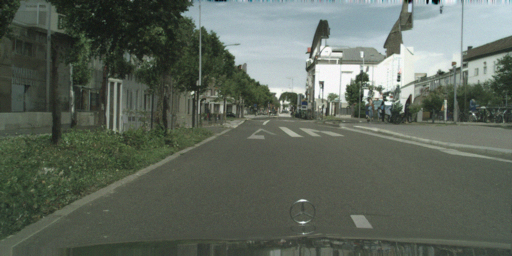
\includegraphics[width=0.25\textwidth]{Chapters/figures/experiments/seg_stop/0_0.8_cond_sample.png} & 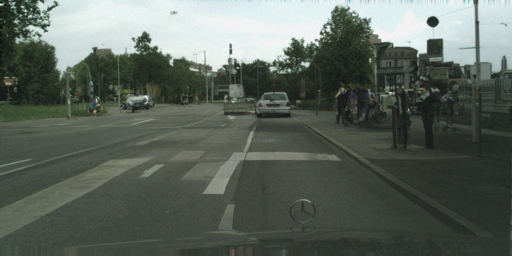
\includegraphics[width=0.25\textwidth]{Chapters/figures/experiments/seg_stop/0_0.7_cond_sample.png} \\
        T=0.65 & T=0.6 & T=0.55 & T=0.5\\
        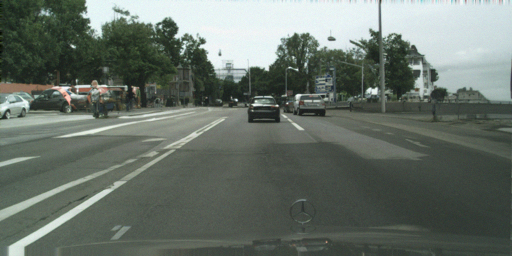
\includegraphics[width=0.25\textwidth]{Chapters/figures/experiments/seg_stop/0_0.6499999999999999_cond_sample.png} & 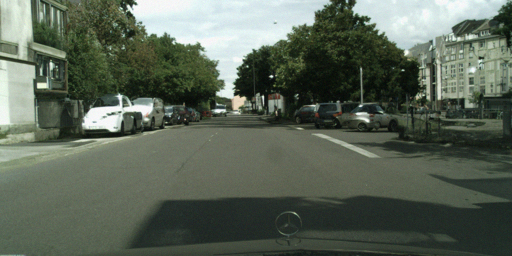
\includegraphics[width=0.25\textwidth]{Chapters/figures/experiments/seg_stop/0_0.6_cond_sample.png} & 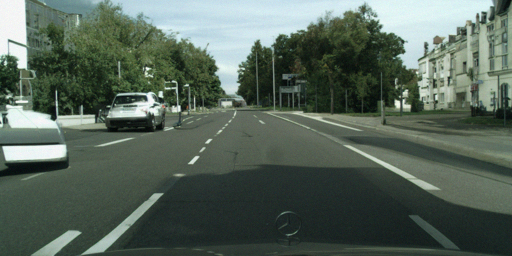
\includegraphics[width=0.25\textwidth]{Chapters/figures/experiments/seg_stop/0_0.55_cond_sample.png} & 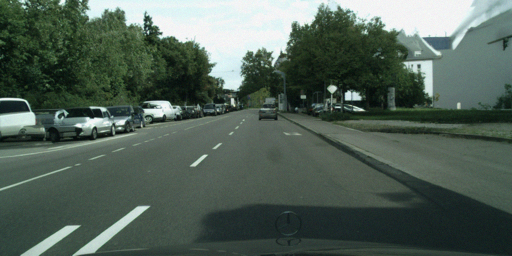
\includegraphics[width=0.25\textwidth]{Chapters/figures/experiments/seg_stop/0_0.5_cond_sample.png}\\
        T=0.45 & T=0.4 & T=0.2 & T=0\\
         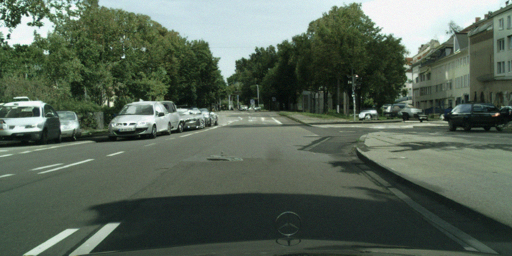
\includegraphics[width=0.25\textwidth]{Chapters/figures/experiments/seg_stop/0_0.44999999999999996_cond_sample.png} & 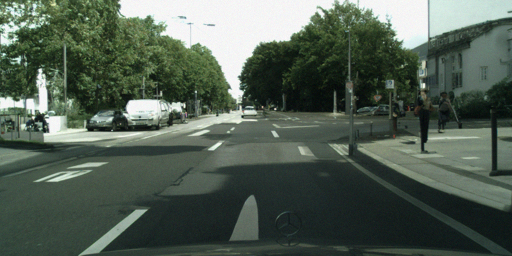
\includegraphics[width=0.25\textwidth]{Chapters/figures/experiments/seg_stop/0_0.3999999999999999_cond_sample.png} & 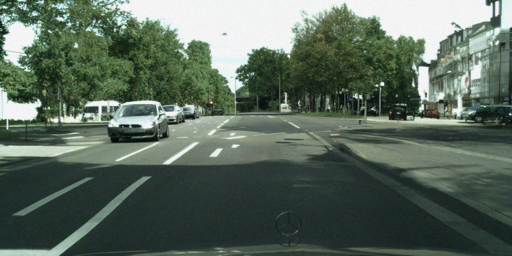
\includegraphics[width=0.25\textwidth]{Chapters/figures/experiments/seg_stop/0_0.19999999999999996_cond_sample.png}& 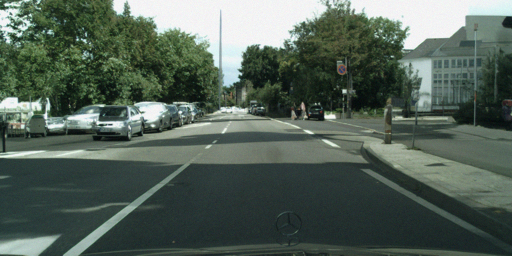
\includegraphics[width=0.25\textwidth]{Chapters/figures/experiments/seg_stop/0_0.0_cond_sample.png} 
    \end{tabular}
    \caption{Stop}
\end{figure}

\begin{figure} \label{fig:5.4}
    \tiny
    \centering
    \setlength\tabcolsep{-2pt}
    \begin{tabular}{cccc}
        Semantic map & Original image & T=0.2 & T=0.4  \\
        \includegraphics[width=0.25\textwidth]{Chapters/figures/experiments/seg_start/0_1.0_seg_mask.png} & 
        \includegraphics[width=0.25\textwidth]{Chapters/figures/experiments/seg_start/0_1.0_original.png} & 
        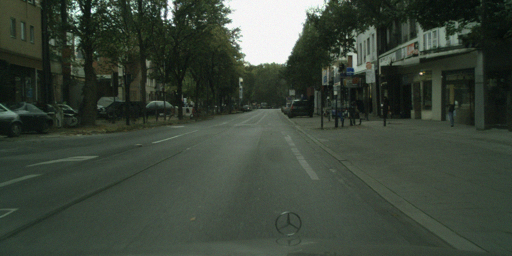
\includegraphics[width=0.25\textwidth]{Chapters/figures/experiments/seg_start/0_0.19999999999999996_cond_sample.png} & 
        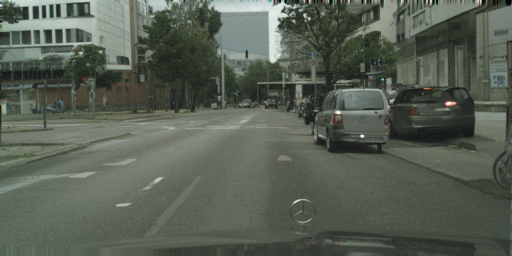
\includegraphics[width=0.25\textwidth]{Chapters/figures/experiments/seg_start/0_0.3999999999999999_cond_sample.png} \\
        T=0.5 & T=0.6 & T=0.65 & T=0.7  \\
        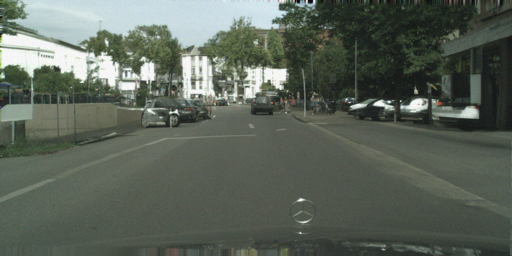
\includegraphics[width=0.25\textwidth]{Chapters/figures/experiments/seg_start/0_0.5_cond_sample.png} & 
        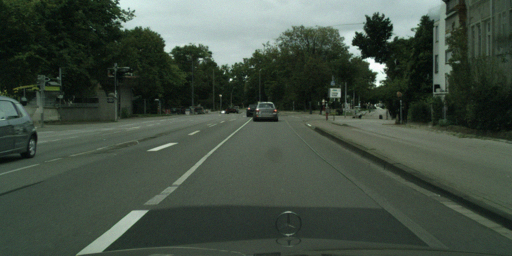
\includegraphics[width=0.25\textwidth]{Chapters/figures/experiments/seg_start/0_0.6_cond_sample.png} & 
        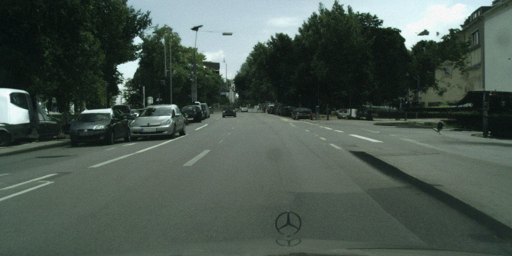
\includegraphics[width=0.25\textwidth]{Chapters/figures/experiments/seg_start/0_0.6499999999999999_cond_sample.png} &
        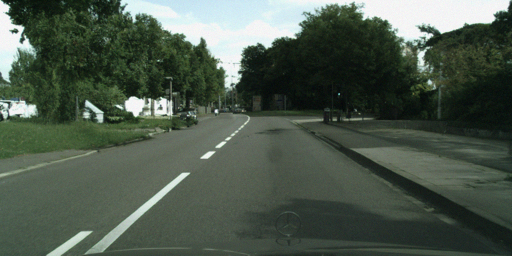
\includegraphics[width=0.25\textwidth]{Chapters/figures/experiments/seg_start/0_0.7_cond_sample.png}  \\
        T=0.75 & T=0.8 & T=0.9 & T=1  \\
        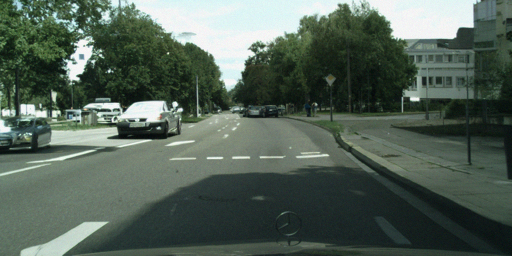
\includegraphics[width=0.25\textwidth]{Chapters/figures/experiments/seg_start/0_0.75_cond_sample.png} & 
        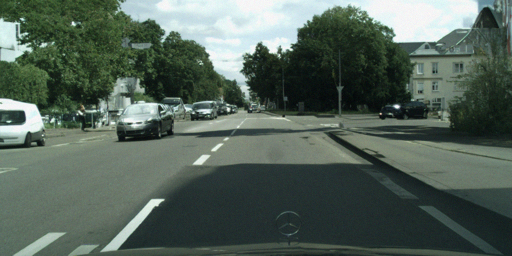
\includegraphics[width=0.25\textwidth]{Chapters/figures/experiments/seg_start/0_0.8_cond_sample.png} & 
        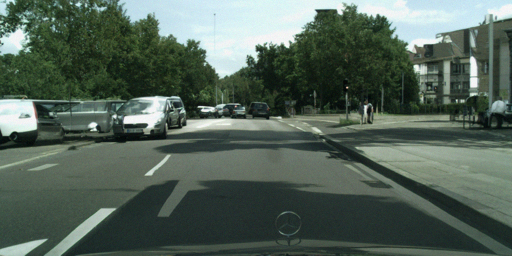
\includegraphics[width=0.25\textwidth]{Chapters/figures/experiments/seg_start/0_0.9_cond_sample.png} & 
        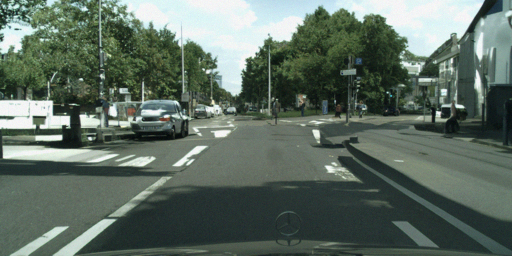
\includegraphics[width=0.25\textwidth]{Chapters/figures/experiments/seg_start/0_1.0_cond_sample.png}
    \end{tabular}
    \caption{Start}
\end{figure}
%%%%%%%%%%%%%%%%%%%%%%%%%%%%%%%%%%%%%%%%%%%%%%%%%%%%%%%%%%%%%%%%%%%%%%%%%%%%%%%%%%%%%%%%%%
\section{Improvements and Adaptations}
As initial experiments before testing semantic image synthesis on a large scale, we test the impact of two improvements/adaptations we made to the original score model architecture \cite{score_3}.
\subsection{Mixed precision learning} %0.5-1
vRAM usage and training speed are key aspects in training deep neural network. Complex models might consist of several million up to billion parameters to optimize. This requires an immense amount of computing power but at least equally important, vRAM. vRAM – video random access memory – is the memory that a GPU has available during operation. Modern high end consumer graphic cards typically have around $10GB$ of vRam. The crux of the matter is that reaching more than $10GB$ when training a moderately complex model is really easy and when training such complex models as NCSNs, the vRAM demand can increase beyond $100GB$, making training deep neural networks a very cost intensive business. Also when training complex models one can expect to need one week or more of training time, making testing and finetuning of models very exhausting.

To mitigate these problems the concept of \textit{Mixed Precision Learning} \cite{mixed_prec} was developed, decreasing both vRAM usage and training time with simultaneous retention of training quality, i.e. training loss. Normally each parameter of a network is stored as a float with $32bits$ of precision. Considering a network with $\sim250M$ parameters this would be equivalent to $\sim1GB$. What sounds not so much at first quickly becomes unmanageable when thinking of the series of matrix arithmetic's the parameters undergo and each calculation storing extra data such as gradients. 

The idea of mixed precision learning is to use floats with a $16bit$ precision wherever possible. In order to not loose model accuracy two concepts are applied. First, there is always a $32bit$ master copy of the model weights. For the forward pass this master copy is converted to $16bit$, where the complex gradient calculations happen. In the backward pass these $16bit$ gradients are converted back to $32bit$ where they are then used by the optimizer to update the master weights. But this improvement during gradient calculation comes with the flaw of loosing some gradients as every number $<2^{-24}$ is equal to $0$ for $16bit$ precision but in most models there is at least some relevant gradient information in the range $[2^{-27},2^{-24})$. To mitigate this effect the concept of loss scaling was proposed. Loss scaling multiplies the $32bit$ loss after the forward pass by a scale factor to move them in the $16bit$ range in which the gradients are then computed in the backward pass. Thereafter the scaled $16bit$ gradients are converted to scaled $32bit$ gradients and then divided by the same scale factor as before. Finally these scaled gradients are used by the optimizer to update the master weights. The full concept can be seen in \hyperref[fig:3.2]{Fig. 3.2}.
%
\begin{figure}[] \label{fig:3.2}
    \centering
    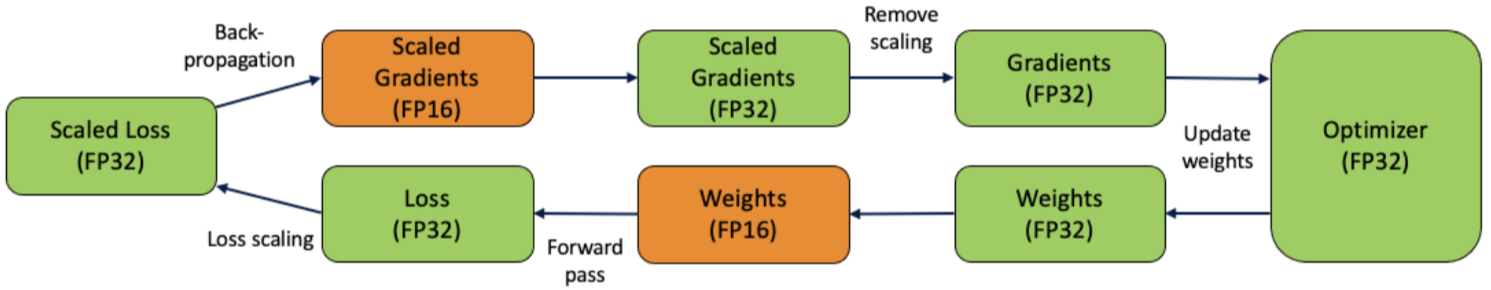
\includegraphics[width=.9\textwidth]{Chapters/figures/mixed_prec.PNG}
    \caption[Short-form caption]{Concept of Mixed Precision}
\end{figure}
%

As the mixed precision technique was not used in the original SGM paper \cite{score_3} it was now implemented using the off the shelf pyTorch tools for mixed precision to check how much this technique improves vRAM usage and training time for the NCSN. To do so we trained the NCSN++ on the Cityscapes dataset on two different GPUs with the same model settings. For each GPU $2\times100$ epochs were passed, once with mixed precision on and once with mixed precision off. The first GPU was a \textit{Nvidia GeForce RTX 2080 Ti} with $11GB$ of vRAM and the second GPU was a \textit{Nvidia A100} with $40GB$ of vRAM. For both GPUs we used the maximum possible batch size for non mixed precision training which is $1$ for the RTX 2080 Ti and $5$ for the A100. The effects of mixed precision training on vRAM usage and training time can be seen in \hyperref[tab:3.1]{Tab. 3.1} resp. \hyperref[tab:3.1]{Tab. 3.2}. For the vRAM usage the total vRAM needed is shown and for the training time the average training time for one epoch is shown.
%
\begin{table}[] \label{tab:3.1}
        \centering
    \begin{tabular}{c|c|c}
        GPU type        & Mixed precision \textbf{Off}    & Mixed precision \textbf{On} \\
        \hline
        RTX 2080 Ti     &  7791MB               & 7367MB\\
        A100            &  39039MB              & 29481MB
    \end{tabular}
    \caption{vRAM usage w/ and w/o mixed precision}
\end{table}
\begin{table}[b] \label{tab:3.2}
        \centering
    \begin{tabular}{c|c|c}
        GPU type        & Mixed precision \textbf{Off}    & Mixed precision \textbf{On} \\
        \hline
        RTX 2080 Ti     &  1494s                & 1206s    \\
        A100            &  965s                 & 987s
    \end{tabular}
    \caption{Training time per epoch w/ and w/o mixed precision}
\end{table}

For the A100 serious improvements on vRAM usage can be observed. For the RTX 2080 Ti there are only little improvements for vRAM usage but good improvements on training time. In general mixed precision is expected to perform way better on the new Ampere GPU
architecture (A100) than on the older Turing GPU architecture (RTX 2080 Ti). To ensure that the training quality does not suffer from the use of mixed precision the loss curves for all test setups are compared in \hyperref[fig:3.3]{Fig. 3.3}. The higher fluctuations for the RTX 2080 Ti are due to the fact that the batch size is smaller, therefore leading to major loss differences in a batch-to-batch comparison. In general it can be seen that mixed precision has no notable effect on training loss. Also a qualitative comparison of generated samples shows no difference perceptible by a human. We therefore conclude that – at least for non FID record breaking attempts – mixed precision should be used and we do so for all upcoming experiments.
%
\begin{figure} \label{fig:3.3}
    \centering
    \begin{subfigure}[b]{0.49\textwidth}
        \centering
         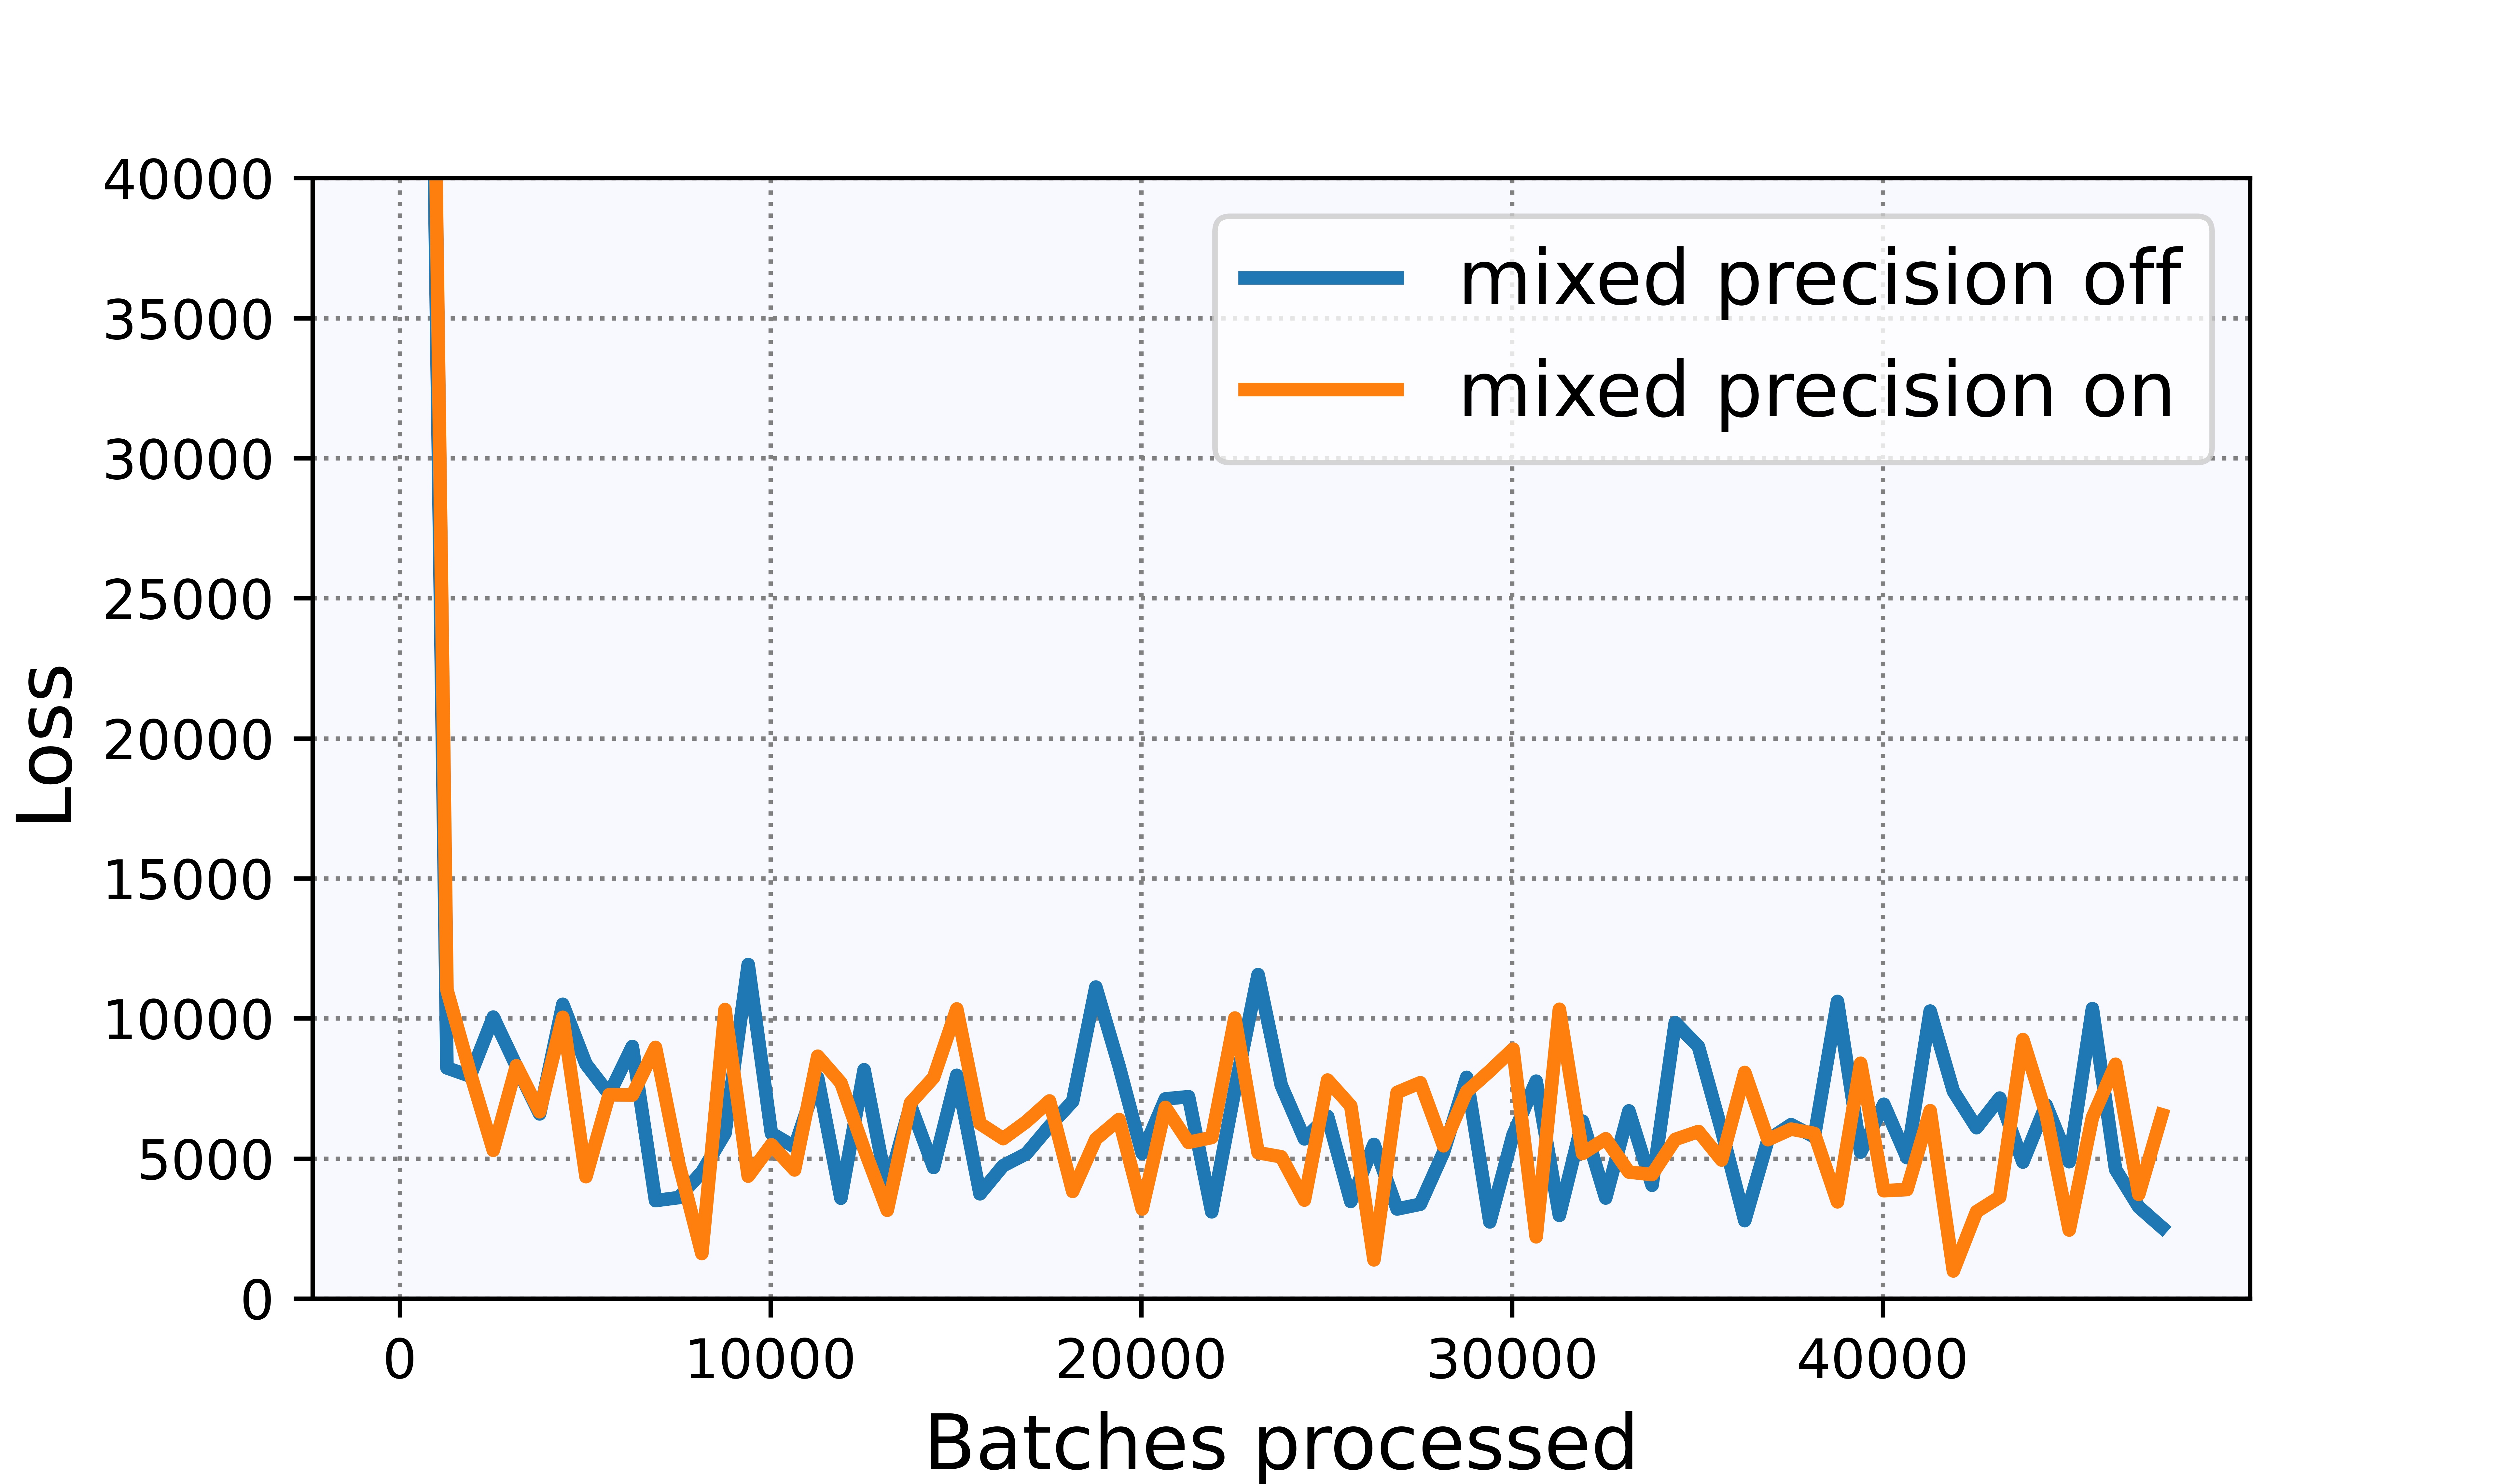
\includegraphics[width=\textwidth]{Chapters/figures/mixed_prec_rtx2080_loss.jpg}
         \caption{Loss curve RTX 2080 Ti}
    \end{subfigure}
    \begin{subfigure}[b]{0.49\textwidth}
        \centering
         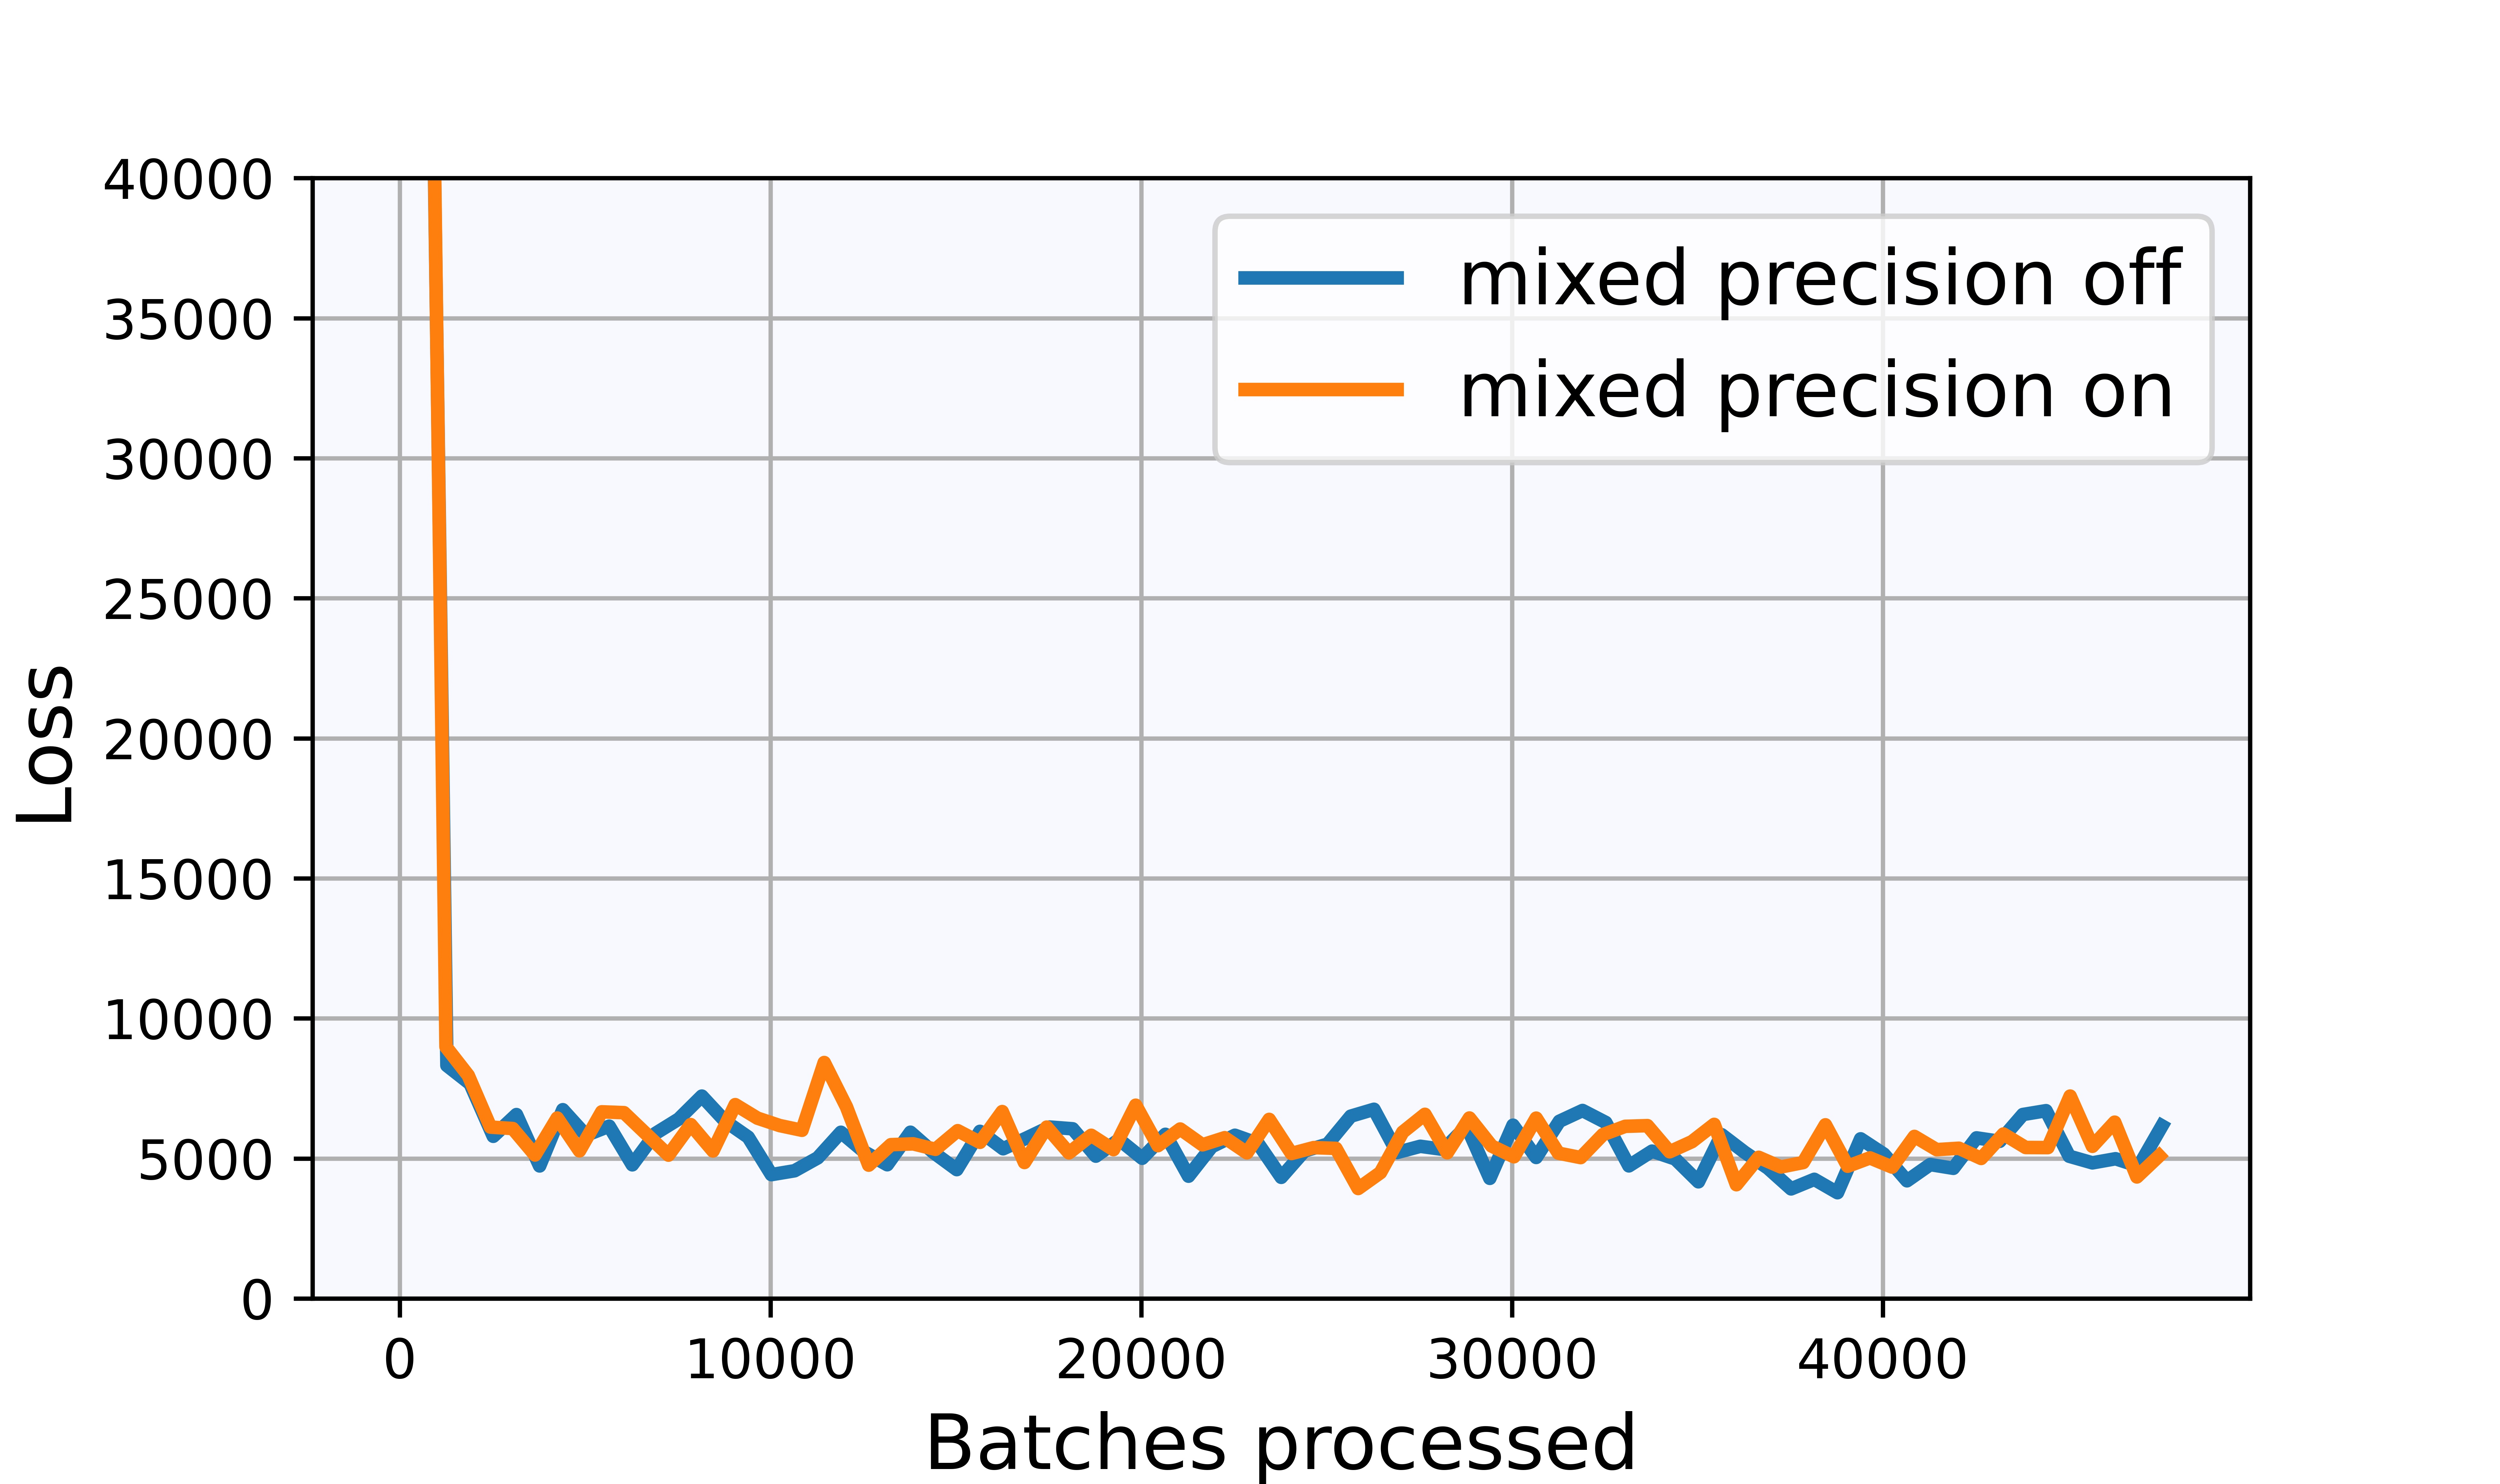
\includegraphics[width=\textwidth]{Chapters/figures/mixed_prec_a100_loss.jpg}
         \caption{Loss curve A100}
    \end{subfigure}
    \caption{Comparing loss curves for mixed precision \textbf{on} an \textbf{off} for both GPUs}
\end{figure}
%
\subsection{Training on arbitrary image sizes} %0.5-1
When training a generative model the image size the model gets as input for learning can have a large effect on what the model learns. Here not the total image size of the images is meant but the image size the model gets as input. As an example the cityscapes dataset (downscaled) consists of $256\times512$ pixel images. To reduce vRAM during training, the images from the dataset often are randomly cropped to another resolution, here $256\times256$. For some datasets this has only little negative effects on the model accuracy, e.g. for landscapes where the relative position of objects to each other only plays a minor role. But for datasets as the cityscapes dataset it is quite important for realistic results that the models learns the logic of images showing street scenes, i.e. learning that the street is in the middle, that there are parking cars on the left and right side of the image and so on. Training on too small crops can hinder the model to learn such logic.

As the version of NCSN \cite{score_3} does not support training on/sampling of non-square images, the model was adapted to do so. Actually the model already was able to process non-square images natively but there was a small bug that we fixed to make non-square training/sampling possible. To show the importance of this bugfix we investigate the influence of the above described effect on NCSN. For this purpose we trained two identical NCSN, one on $256\times256$ crops and one on the $256\times512$ original images. Some example results can be seen in \hyperref[tab:5.3]{Tab.\,5.3}. It is clearly visible that the full image model outperforms the cropped image model when the focus of evaluation is on street scene logic. It must be mentioned that for semantic image synthesis – the task for our experiments – this logic information actually is given by the semantic map which initially gives rise to the idea of training on crops at all. Nevertheless we suspect that a model knowing the logic without a semantic map also performs somewhat better than if it did not. For that reason models for further experiments on the cityscapes dataset were always trained with the full size images.
\begin{table}[] \label{tab:5.3}
    \centering
    \setlength\tabcolsep{-2pt}
    \begin{tabular}{ccc}
        & Training size $256\times256$ & \\
        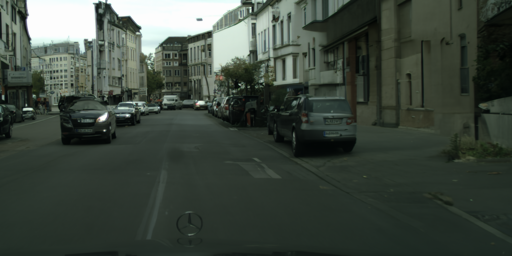
\includegraphics[width=0.33\textwidth]{Chapters/figures/experiments/crop/1_sample.png} &
        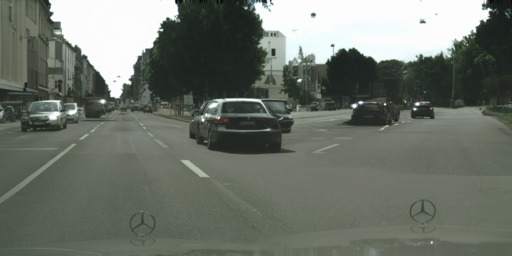
\includegraphics[width=0.33\textwidth]{Chapters/figures/experiments/crop/5_sample.png} &
        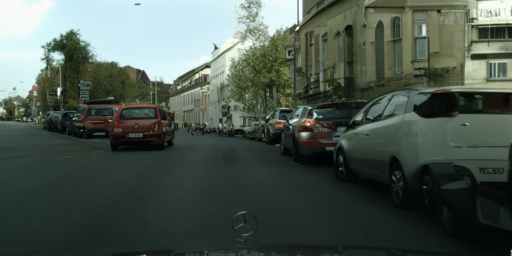
\includegraphics[width=0.33\textwidth]{Chapters/figures/experiments/crop/8_sample.png}\\
        & Training size $512\times256$ & \\ 
        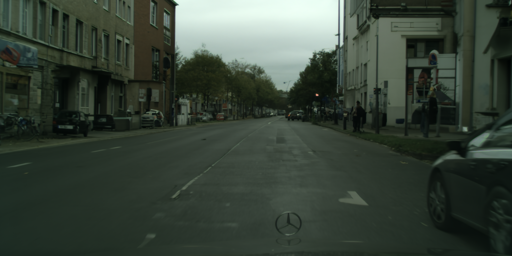
\includegraphics[width=0.33\textwidth]{Chapters/figures/experiments/crop/0_uncond_sample.png} &
        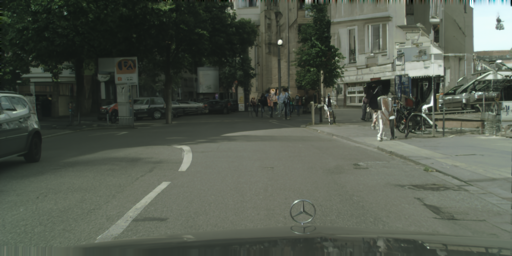
\includegraphics[width=0.33\textwidth]{Chapters/figures/experiments/crop/3_uncond_sample.png} &
        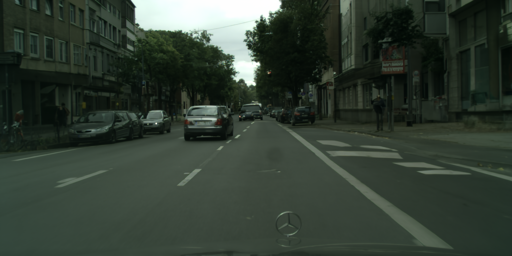
\includegraphics[width=0.33\textwidth]{Chapters/figures/experiments/crop/7_uncond_sample.png}
    \end{tabular}
    \caption{Unconditional example images of NCSN trained on cropped images (\textit{top}) and full size images (\textit{bottom}).}
    \label{tab:my_label}
\end{table}

%%%%%%%%%%%%%%%%%%%%%%%%%%%%%%%%%%%%%%%%%%%%%%%%%%%%%%%%%%%%%%%%%%%%%%%%%%%%%%%%%%%%%%%%%%%%%%%%%

\section{A competitive experiment on the Cityscapes dataset} \label{sec:5.4}

\subsection{The Cityscapes dataset}
\subsection{Metrics}

\section{Synthesizing high resolution landscapes} \label{sec:5.5}


